\section{Problem Formulation}
\label{sec:problemformulation}

In this section, we formulate the problem of band selection in wireless 
mesh network deployment jointly using WiFi and white space bands. 
We first illustrate the challenges of band selection
in deploying wireless network. Then we discuss the number of access
 points estimation in deploying wireless mesh network. Finally, we present 
measurement driven estimation framework to address the problem. 
 
\subsection{White Space Opportunity and Challenge}
\label{subsec:motivation}
Wireless communication have changed the world since the day it was discovered.
Today, wireless signals fill up the world across all the frequency bands.
These signals help people improving their lives but also bring interference to each other.
In any topic of wireless communication, the interference of existed signals
 have to be considered as an important part.  Such as yielding primary users
is a key issue in cognitive radio~\cite{haykin2005cognitive}. Researchers have 
put many efforts in solving issues of wireless network in gateway deployment, channel 
assignment, routing, etc.~\cite{he2008optimizing,tang2005interference}.
Most of the works in wireless network solutions assume the channels are clean 
which unfortunately is not true.

The interference of a wireless network could be divided into two catalog according
 to the interference source.
 One is the {\it Intra-network intereference} which the nodes in the 
network interference each other. The other {\it Inter-network interference}
 is from signal sourse who is not in the network. 
The assumption make the recent works of wireless 
network deployment focus on the allocation of intra-network interference~\cite{si2010overview}. 
However, the omits of inter-network interference becomes an problem when 
white space bands come in to data communication. The inter-network 
interference of TV station and other signal source need to be 


HERE FIXME

. 



% Propagation

Wireless propagation is the behavior of the signal loss characteristics 
when wireless signals are transmitted in the medium, most of the time in the air.
The strength of the receiving signal depends on both the line-of-sight
path (or lack thereof) and multiple other paths that are a result of 
reflection, diffraction, and scattering from obstacles in the 
environment~\cite{andersen1995propagation}. The widely-used, Friis
equation characterizes the power of the received signal $P_r$ in terms 
of the power $P_t$ and gain $G_t$ of the transmitting signal, gain of 
the receiver $G_r$, wavelength $\lambda$ of the carrier frequency, 
distance $R$ from transmitter to receiver, and path loss exponent $n$ according 
to~\cite{friis}:
\begin{equation}
\label{eq:friis}
P_r=P_t+G_t+G_r+10n \log_{10}\left( \frac{\lambda}{4\pi R}\right)
\end{equation}
Here, the path loss exponent $n$ varies according to the
aforementioned environmental factors and ranges from 2 to 5 in typical
outdoor settings~\cite{rappaport}.

% Explain multiband and activity level
Before FCC release white space bands, the channel separation is relatively 
small (e.g., 22 MHz for the 2.4 GHz band), many works assume the propagation 
of these channels are the same which match the restriction. 

Here, a frequency band is defined as a group of channels which have
similar propagation characteristics.
Moreover, the activities in multiple bands vary from downtown area 
to rural area due to the distribution of TV stations, wireless instrument. More 
activities of WiFi bands may be observed in neighborhood. More white space band
 activities could be observed than WiFi activities in rural area. 
This characteris bring more options for band selection in WiFi and white space.
In this work, we consider the diverse propagation and activity characteristics
for four total frequency bands: 450 MHz, 800 MHz, 2.4 GHz, and 5.2 GHz.
The two former frequency bands, we refer to as white space (WS) bands whereas
the two latter frequency bands, we refer to as WiFi bands.


% Network Constraint
There are several constraints for deploying wireless mesh network. In backhual tier 
connectivity constraint requires all clients could be connected to access points.
When access points locations are unknown or not yet selected, the possible access points
 need to cover all the area with a coverage constraint. We assume the coverage
constraint is $95\%$ for a target area~\cite{robinson2010deploying}. 
Moreover, wireless bandwidth is shared amongst all clients, which is desirable to 
limit the number of potential shares of the scarce wireless spectrum. Spacial reuse 
helps to improve the capacity constraint. When an access point is serving an area, it has
to satisfy the demand of the residents. We hold the residents demand as capacity constraint.

% Make multiband challenges
Avoiding interference is the primary target in wireless deployment.
Previous work focus on resolve the Intra-network 
interference~\cite{subramanian2008minimum,ramachandran2006interference,si2010overview}.
Due to the distribution nature of the Inter-network interference,
it is impossible to have a theoretic model to describe and estimate the activities of existing
 wireless signals. Measurement is the best and probably the only way to tell the Inter-network
  interference. The broadcast nature of the wireless medium make greater levels of propagation 
  induce higher levels of interference, both for Inter-network
and Intra-network interference. To smart use of WiFi and white space band adapting different 
demands of rural area and urban areas is a key issue in wireless network. 
Thus, in sparsely-populated rural areas, the lower frequencies of the white space 
bands might be a more appropriate choice for wireless service in huge sparse areas. 
However, as the population and demand scales up (e.g., 
for more urban regions), the reduced spatial reuse and greater levels of Inter and Intra interference 
of white space bands might detract from the overall deployment strategy. In 
such urban areas, select links of greater distance might be the most 
appropriate choice for white space bands, especially since the number of 
available channels is often inversely proportional to the population (due 
to the existence of greater TV channels).
%The broadcast nature of the wireless medium makes it generate multiple access interference in wireless network.
%Employing White Space Band in lower frequency brings advantages for mesh network, 1) more orthogonal bandwidth reduce the contention and conflict in the network,
% 2) the propagation variation brings flexible topology by reducing connection hop counts in the network.
%However, at the same time, links in White Space Band also increase the interference range in the network making space reuse of the white space band channel difficult. 


The distribution of inter-network interference vary in downtown, urban and rural area.
We did measurement driving through Dallas, Fort Worth, and Weatherford in north Texas as shown in Figure~\ref{fig:drivemap}.
The spectrum measurement is shown in Figure~\ref{fig:drivetest}.
The signal strength of 450 MHz is strong in downtown Dallas, downtown Fort Worth;
but has less interference in the urban and rural area between these cities.
The low variation of 5.2 GHz and 2.4 GHz due to the limited transmitting range.
When we drive in the highway, the distance from our car to the weak signal source of these bands
is to large to detect these signals. We did more fixed location measurement to quantify
the spacial distribution. 
   \begin{figure}
   %\vspace{-0.0in}
   \centering
   \includegraphics[width=74mm]{figures/drivemap}
   \vspace{-0.1in}
   \caption{DFW Drive Test Map}                                                                 
   \label{fig:drivemap}
   %\vspace{-0.0in}
   \end{figure}
   
   
   \begin{figure}
   %\vspace{-0.0in}
   \centering
   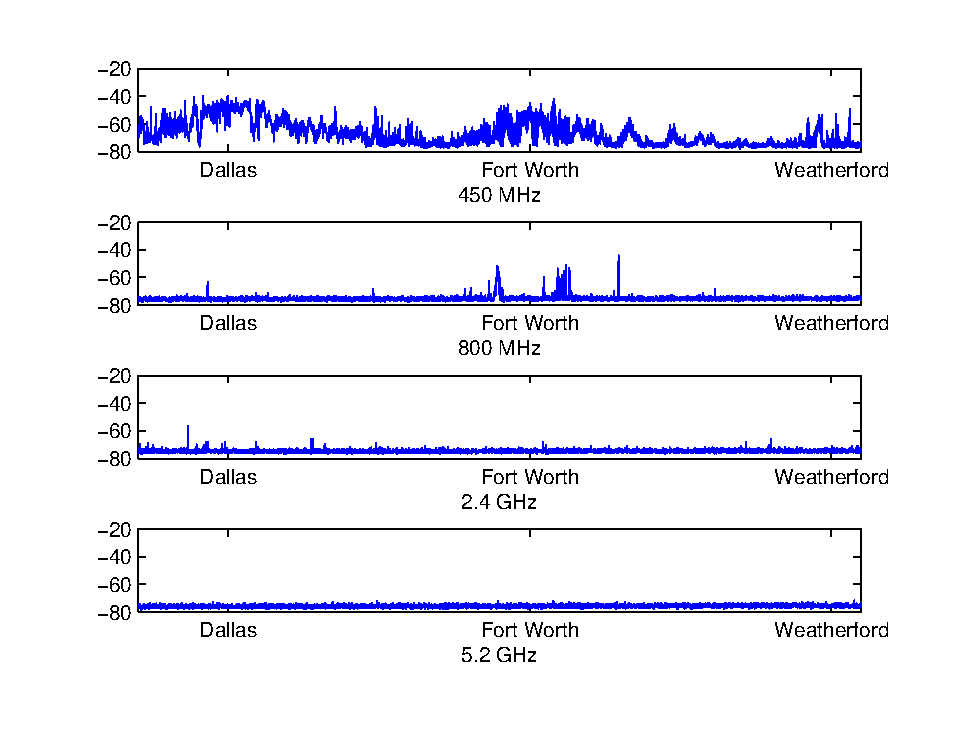
\includegraphics[width=74mm]{figures/drivetest}
   \vspace{-0.1in}
   \caption{Spectrum Activity In DFW}                                                                 
   \label{fig:drivetest}
   %\vspace{-0.0in}
   \end{figure}

We define measured percentage activity time in a unit time to 
quantify the Inter-network interference~\ref{subsec:problem}.
Figure \ref{fig:labact} depicts an example activity level in our urban lab
with the platform introduced in~\ref{sec:experimentdesign}. 
The interference across varies in time domain. The activity level from data
collected in the same location shows the difference in time domain.
The existing signals occupy 25.83 percentage of time in 450 MHz,
26.49 percentage of time in 800 MHz, 34.95 percentage of time in 
2.4 GHz and 35.46 of time in 5.2 GHz. The Inter-network interference 
of these existing signals is what we have to avoid in wireless network
 deployment. 
   \begin{figure}
   %\vspace{-0.0in}
   \centering
   \includegraphics[width=74mm]{figures/labactivity}
   \vspace{-0.1in}
   \caption{Wireless Activity in Urban Lab}                                                                 
   \label{fig:labact}
   %\vspace{-0.0in}
   \end{figure}
There is around $10\%$ difference from white space band to WiFi band in 
our lab. This gap is an opportunity to improve wireless network deployment.
%To balance the larger communication range and interference range of white space band in mesh network is a key issue in ~\emph{Multiband Mesh Network} from ~\emph{Multiradio} scenario.

\subsection{Model and Problem Formulation}
\label{subsec:problem}

% Assumptions of the network
Oppose to previous works, this paper focus on bands adaptation of Inter-network 
interference and multiple populated areas~\cite{tang2005interference,yuan2006cross
,si2010overview}. We propose a measurement driven framework to get the lower bound 
amount of access points for serving a certain area with QoS requirement.
 We hypothesize that using radios with a greater diversity in propagation could 
 achieve overall network performance gains.  Therefore, for a given set of radios,
  we allow the channel choices to come from different frequency bands 
  (i.e., multiband channel assignment). We assume that all mesh nodes have the same 
  transmit power, channel bandwidth, and antenna gain.
Each access point operates with a classic protocol model~\cite{gupta2000capacity}. 

Generally, Internet data request comes with population and Finland government even announce 
broadband is an individual 'legal right'~\cite{bbcfinland,rosston2011household}. Providing a community 
wireless Internet service have to satisfy its traffic demand of multiple population distribution. 
Figure ~\ref{fig:dfwpopulation} depicts the population distribution of Dallas-Fort Worth 
metropolitan area. Population increase with red color and decrease with green color in the map.
In populated urban area, more people need more network capacity in which case WiFi 
band spatial reuse is better than white space band who limit its capacity in one NIC for the whole area.
However, in populated urban area, more Inter-network interference comes from existing devices in WiFi
 bands could reduce the capacity of a spatial reuse WiFi network. 
 Here we are trying to answer the question in a certain Inter-network interference,
 what is the band or bands combination we should use to provide network service
  for a community.
	  
   \begin{figure}
   %\vspace{-0.0in}
   \centering
   \includegraphics[width=84mm]{figures/experimentloc}
   \vspace{-0.1in}
   \caption{Dallas-Fort Worth Population Distribution}                                                                 
   \label{fig:dfwpopulation}
   %\vspace{-0.0in}
   \end{figure}

Since mathematical formula is difficult to describe the activities of signal on the air even in an arbitrary area.
 We use long term measurement represent the activities in each band is a good
  estimation. We define the the percentage of sensing samples $S_\theta$ above a 
  interference threshold $\theta$ over the total samples $S$ in a time unit as the 
  {\it $Activity Level$} $A$ of Inter-network interference shown in equation~\ref{eq:actdef}
\begin{equation}
\label{eq:actdef}
A=\frac{S_\theta}{S_a}
\end{equation}
The capacity of a clean channel is $C$, with protocol model, the capacity of a channel with Inter-network
 interference $C_r$ could be represented as in equation~\ref{eq:intercap}
\begin{equation}
\label{eq:intercap}
C_r=C*(1-\bar{A})
\end{equation}

The lower bound of a network deployment is to provide network capacity equal to the demand of the service 
area. The demand of a service area could be calculated as the summation of individual demand all over 
the service area $D_a=\sum_{p\in P}D_p$. Since individual or family Internet data demand is marked as government 
statistics~\cite{rosston2011household}, $D_a$ could be remarked with population distribution $f$ and service area $k$ as 
$D_a=\sum_{f \in F,k \in K}\bar{D_p}*f*k$. The network deployment lower bound of access point $M$ could be 
represented in equation~\ref{eq:nlbound}

\begin{equation}
\label{eq:nlbound}
\sum_{m \in M}C_r^m \ge \sum_{f \in F,k \in K}\bar{D_p}*f*k
\end{equation}
Also, the network has to satisfy the coverage constraint. The access tier provides 
single-hop connectivity from client devices to a mesh node. 
Generally a coverage of $95\%$ is good for outdoor mesh network~\cite{robinson2010deploying}.

In multiband scenario, the activity level varies with to different interference source and the propagation
 characteristics bring the service area variation. The simplest way to cover an area is to use 
 multiple orthogonal lower frequency channels, however, FCC limit the white space band utility in 
 most metro area in US~\cite{googledatabase}. Moreover, channel in each band is limited. 
 And too many lower frequencies channels will bring  huge Intra-network interference for 
 the network which is out of our scope. To answer the question given an area for a new network, 
 at least how many access point or how much funding should be risen, we build the measurement driven
  framework to approach the lower bound.




% Fix the framework , Mark should use them in a single tower with more radios
% Framework
In space domain, the advantage of high frequency channel in network is the spatial reuse, the low
frequency channel is better in large scale coverage. Generally high frequency fit
for populated area and low frequency fit for sparse area.
The time domain variation could be seen in Figure~\ref{drivetest}.
For an ISP, the service quality which maps to the capacity constraint has to be satisfied.
Given an area of metropolitan, the population distribution could be found in 
government and academy resources~\cite{uscensus}. Then we have the capacity request
of each part of the area with the assumption everyone has the same Internet demand. 
According to the population distribution, we chop the area into different types.
These are the space domain input. Then we count the measured activity level as 
input in time domain. We have an average channel capacity of each band with the 
activity level. With received signal strength threshold, 
the QoS coverage area of different type per channel and the reuse distance could be computed. 
Then the maximum area an access point could cover can be calculated as the minimize 
area of the QoS coverage area and propagation coverage.
Then the transmitting power is adjusted to fulfill the coverage restriction. 
A classic regular hexagon deployment process is employed to put the access points.


% Fixme think about the framework
%\subsection{Measurement Driven Access Point Lower Bound Approaching Framework}
%\label{subsec:MDLB}
%
\begin{algorithm}[t]
    \small
\caption{Number of Access Points Estimation}
\label{algorithms:bps}
\begin{algorithmic}[1]
\REQUIRE  ~~\\
	$A$: Measured Activity Level \\
	$F$: Population Distribution\\
	$C$: Clean Channel Capacity\\
	$n$: Path Loss Exponent \\
	$B$: Available frequency bands\\
	$M$: Area need to be covered
\STATE Chop $M$ in to different type, calculate the traffic demand density $f$
\STATE Calculate in-field channel capacity $C_r$ as $C(1-A)$  
\STATE Get the propagation coverage area radius $R_p$ from Frii model based on $n,B,F$
\STATE Calculate the QoS coverage radius $R_{QoS}$ of a Multiband Access Point satisfy the demands of the area
\STATE The coverage radius of a Multiband Access Point is $Min{R_p,R_{QoS}}$
\STATE Apply regular hexagon deployment to get the number of access point for serving given area $M$ 
\ENSURE ~~\\    
 The number of Access Points\\
\end{algorithmic}
\end{algorithm}

With this framework, we combine our measurement and public population data to evaluate white
 space band application in dense populated area, sparse area in section~\ref{sec:experimentdesign}.



